\documentclass[11pt]{article}
\usepackage[a4paper,margin=0.88in]{geometry}
\usepackage{amsmath,amssymb,amsthm,mathtools}
\usepackage{booktabs,array}
\usepackage{graphicx}
\usepackage{xcolor}
\usepackage[hidelinks]{hyperref}
\hypersetup{
  pdftitle={Proper-Delay Spectra Majorize Subspace Rotation},
  pdfauthor={Lluis Eriksson},
  pdfsubject={Sharp Ky Fan quantum speed limits for passive networks}
}
\usepackage[nameinlink,capitalise]{cleveref}
\usepackage{microtype}

\newtheorem{theorem}{Theorem}[section]
\newtheorem{proposition}[theorem]{Proposition}
\newtheorem{lemma}[theorem]{Lemma}
\newtheorem{corollary}[theorem]{Corollary}
\theoremstyle{definition}
\newtheorem{definition}[theorem]{Definition}
\newtheorem{example}[theorem]{Example}
\theoremstyle{remark}
\newtheorem{remark}[theorem]{Remark}
\newtheorem{limitation}[theorem]{Limitation}

\newcommand{\C}{\mathbb C}
\newcommand{\T}{\mathbb T}
\newcommand{\tr}{\operatorname{tr}}
\newcommand{\ran}{\operatorname{ran}}
\newcommand{\diag}{\operatorname{diag}}
\newcommand{\dd}{\mathrm d}
\newcommand{\e}{\mathrm e}
\newcommand{\Spr}{\operatorname{Spr}^{+}}
\newcommand{\KF}{\operatorname{KF}}
\newcommand{\mcdeg}{\deg_{\mathrm{McM}}}
\newcommand{\opnorm}[1]{\lVert#1\rVert_{\mathrm{op}}}
\newcommand{\pos}[1]{\left[#1\right]_{+}}

\title{Proper-Delay Spectra Majorize Subspace Rotation:\\
Sharp Ky Fan Quantum Speed Limits for Passive Networks}
\author{Lluis Eriksson}
\date{10 August 2026}

\begin{document}
\maketitle

\begin{abstract}
A subspace quantum speed limit usually records only the largest canonical
angle.  Passive scattering theory usually records either the largest proper
delay or their total trace.  Both compressions discard how a rank-$k$ routing
event is distributed across modes.  We derive the missing vector law.  If
$S(t)\in U(N)$ is absolutely continuous,
$Q(t)=-\mathrm iS(t)^*\dot S(t)$ is its Hermitian generator, and
$\beta_1\geq\cdots\geq\beta_k$ are the canonical angles between a fixed
rank-$k$ subspace and its transported image, then, for every
$r\leq\min\{k,N-k\}$,
\[
 2\sum_{j=1}^r\beta_j
 \leq \int\sum_{j=1}^r
 \bigl(\lambda_j(Q)-\lambda_{N-j+1}(Q)\bigr)\,\dd t .
\]
Thus the integrated spectral-spread vector weakly majorizes twice the
canonical-angle vector.  For a positive Wigner--Smith flow this yields a
hierarchy in the $r$ leading proper delays; $r=1$ recovers the bandwidth-type
subspace limit, while $r=k$ strengthens the trace-action law.  Every partial
sum is simultaneously sharp for every prescribed angle spectrum.  An exact
nonnegative slack decomposition separates three causes of inefficiency:
common-mode delay, failure to use the available spectral spread, and a
nongeodesic subspace path.  Robust corollaries turn heterogeneous pass/stop
leakage spectra and operator-norm tomography errors into certified Lorenz
curves for delay and, for rational inner networks, McMillan-degree lower
bounds.  The matrix spectral-spread inequality and Grassmann metrics used in
the proof are established results; the contribution is their dynamical
composition with Wigner--Smith positivity, robust routing data and realization
degree.  A deterministic artifact tests 8,192 random generators, 1,536 random
time-dependent paths, sharp equality families and 2,048 noisy tomography
instances.  Source, frozen data and independent replay are available in the
\href{https://github.com/lluiseriksson/finite-sample-spectral-certificates/releases/tag/v1.4-ky-fan-speed-limits}{immutable companion release}.
\end{abstract}

\noindent\textbf{Keywords:} quantum speed limit; Wigner--Smith time delay;
canonical angles; weak majorization; Ky Fan norm; passive quantum network;
McMillan degree; robust spectral routing.

\section{One routing event, an entire Lorenz curve}

Suppose that a device moves a $k$-dimensional family of inputs through output
space.  A scalar description asks only how far the worst direction moved, or
sums all motion and all delay.  Neither distinguishes a coherent rotation of
all $k$ directions from one violently delayed direction accompanied by
$k-1$ nearly stationary ones.  The distinction matters in multiport filters,
frequency-selective reservoirs and passive quantum networks.

The correct statement is vector-valued.  Write the ordered endpoint angles as
$\beta=(\beta_1,\ldots,\beta_k)$.  Write the ordered eigenvalues of the
instantaneous generator as $\lambda_1(Q)\geq\cdots\geq\lambda_N(Q)$, and set
\begin{equation}\label{eq:spreadvector}
 \Spr_j(Q)=\lambda_j(Q)-\lambda_{N-j+1}(Q),\qquad
 1\leq j\leq\lfloor N/2\rfloor.
\end{equation}
Our central law is
\begin{equation}\label{eq:headline}
 2\beta\ \prec_w\ \int \Spr(Q(t))\,\dd t,
\end{equation}
with both vectors truncated to $m=\min\{k,N-k\}$.  Here $x\prec_w y$ means
$\sum_{j=1}^r x_j\leq\sum_{j=1}^r y_j$ for every prefix $r$.
The hierarchy is invariant under $Q(t)\mapsto Q(t)+c(t)I$: common phase does
not rotate a subspace.

For a passive monotone scattering path, $Q\succeq0$ and its eigenvalues are
the proper delays.  Since every bottom partial sum is nonnegative,
\begin{equation}\label{eq:properdelayheadline}
 2\sum_{j=1}^r\beta_j
 \leq \int\sum_{j=1}^r\Spr_j(Q)\,\dd t
 \leq \int\sum_{j=1}^r\lambda_j(Q)\,\dd t.
\end{equation}
The first inequality says that no collection of fewer than $r$ large proper
delays can hide a collective rotation of the first $r$ canonical directions.
The full list of prefix inequalities is a Lorenz-curve certificate.

The result refines the preceding robust routing law
\cite{ErikssonRouting2026}.  That work proved only the endpoints $r=1$ and a
trace bound at $r=k$.  Here every intermediate $r$ is controlled, the
generator need not be positive for the spectral-spread theorem, heterogeneous
directional leakage is retained rather than collapsed to one tolerance, and
an exact slack identity diagnoses near saturation.

Our claims are deliberately separated from the ingredients.  Unitarily
invariant Grassmann metrics are due to Qiu, Zhang and Li
\cite{QiuZhangLi2005}.  The sharp block inequality
$2s(B)\prec_w\Spr(Q)$ and its constant-generator subspace consequence were
proved by Massey, Stojanoff and Z{\'a}rate
\cite{MasseyStojanoffZarate2021}.  Maximal-angle subspace speed limits are
known from Albeverio and Motovilov
\cite{AlbeverioMotovilov2022a,AlbeverioMotovilov2022b}; geometric operator
speed limits and bandwidth-constrained transformations provide neighboring
frameworks \cite{AllanHornedalAndersson2021,CarabbaEtAl2022,HornedalEtAl2023}.
The new result here is the complete time-dependent partial-sum law and its
operational consequences for positive Wigner--Smith spectra, robust
tomography, exact memory accounting and rational realization degree.

\section{Geometry and generators}

Let $S:[a,b]\to U(N)$ be absolutely continuous and define
\begin{equation}\label{eq:generator}
 Q(t)=-\mathrm iS(t)^*\dot S(t).
\end{equation}
Then $Q(t)$ is Hermitian almost everywhere and
$\dot S(t)=\mathrm iS(t)Q(t)$.  Fix a rank-$k$ projection $P_0$ and let
\begin{equation}
 \mathcal X(t)=\ran(S(t)P_0),\qquad
 \Pi(t)=S(t)P_0S(t)^*.
\end{equation}
Let $\beta_1\geq\cdots\geq\beta_k\in[0,\pi/2]$ be the canonical angles
between $\mathcal X(a)$ and $\mathcal X(b)$.  Only
$m=\min\{k,N-k\}$ can be nonzero.

Relative to $\ran P_0\oplus\ran(I-P_0)$, write
\begin{equation}\label{eq:blockQ}
 Q(t)=\begin{bmatrix}A(t)&B(t)^*\\B(t)&C(t)\end{bmatrix},
 \qquad B(t)=(I-P_0)Q(t)P_0.
\end{equation}
The diagonal blocks change phases inside the two instantaneous sectors.  The
horizontal block $B$ alone moves the point of the Grassmannian.  Let
$s_1(B)\geq\cdots\geq s_m(B)$ be its singular values and define the Ky Fan
velocity
\begin{equation}
 \nu_r(B)=\sum_{j=1}^r s_j(B),\qquad 1\leq r\leq m.
\end{equation}

\begin{lemma}[Grassmann path length]\label{lem:path}
For every $1\leq r\leq m$,
\begin{equation}\label{eq:pathlength}
 \sum_{j=1}^r\beta_j\leq\int_a^b\nu_r(B(t))\,\dd t.
\end{equation}
\end{lemma}

\begin{proof}
For the symmetric gauge $\Phi_r(x)=\sum_{j=1}^r x_j^\downarrow$,
$d_r(\mathcal U,\mathcal V)=\Phi_r(\Theta(\mathcal U,\mathcal V))$ is a
unitarily invariant Grassmann metric \cite{QiuZhangLi2005}.  The metric
derivative of $\mathcal X(t)$ is $\Phi_r(s(B(t)))$: conjugating
$\dot\Pi=\mathrm iS[Q,P_0]S^*$ back by $S$ leaves the horizontal tangent
block $B$.  The distance between endpoints does not exceed the length of an
absolutely continuous path, which is exactly \eqref{eq:pathlength}.
\end{proof}

\section{The Ky Fan speed-limit hierarchy}

The algebraic bridge is a sharp result from
\cite[Theorem~2.7]{MasseyStojanoffZarate2021}.  We restate it in the notation
needed for the dynamical argument and include a short Ky Fan proof.

\begin{lemma}[Spectral-spread block inequality]\label{lem:block}
Let $Q=Q^*$ have the block form \eqref{eq:blockQ}.  For every
$1\leq r\leq m$,
\begin{equation}\label{eq:blockspread}
 2\sum_{j=1}^r s_j(B)
 \leq\sum_{j=1}^r\bigl(\lambda_j(Q)-\lambda_{N-j+1}(Q)\bigr).
\end{equation}
The constant $2$ is optimal.
\end{lemma}

\begin{proof}
Put $J=2P_0-I$.  Then
\[
 Q-JQJ=2\begin{bmatrix}0&B^*\\B&0\end{bmatrix},
\]
whose $r$ largest eigenvalues are $2s_1(B),\ldots,2s_r(B)$.
Ky Fan's eigenvalue inequality \cite{Fan1951} applied to
$Q+(-JQJ)$ gives
\[
 \sum_{j=1}^r\lambda_j(Q-JQJ)
 \leq\sum_{j=1}^r\lambda_j(Q)+\sum_{j=1}^r\lambda_j(-JQJ).
\]
Unitary conjugation preserves the spectrum and
$\lambda_j(-Q)=-\lambda_{N-j+1}(Q)$, proving \eqref{eq:blockspread}.
Sharpness follows already for $Q=\bigl[\begin{smallmatrix}0&B^*\\B&0\end{smallmatrix}\bigr]$.
\end{proof}

\begin{theorem}[Time-dependent spectral-spread QSL]\label{thm:main}
Let $S$, $Q$, $P_0$ and $\beta$ be as above.  Then for every
$1\leq r\leq m$,
\begin{equation}\label{eq:main}
 \boxed{\quad
 2\sum_{j=1}^r\beta_j
 \leq\int_a^b\sum_{j=1}^r
 \bigl(\lambda_j(Q(t))-\lambda_{N-j+1}(Q(t))\bigr)\,\dd t.
 \quad}
\end{equation}
Equivalently, $2\beta\prec_w\int_a^b\Spr(Q(t))\dd t$, after
truncation to $m$ entries.  The theorem is invariant under an arbitrary
time-dependent scalar shift of $Q$.
\end{theorem}

\begin{proof}
Apply \cref{lem:block} almost everywhere, integrate, and combine with
\cref{lem:path}.  Both sides of \eqref{eq:main} are unchanged by
$Q(t)\mapsto Q(t)+c(t)I$.
\end{proof}

\begin{corollary}[Positive proper-delay hierarchy]\label{cor:positive}
If $Q(t)\succeq0$ almost everywhere, then for every $r\leq m$,
\begin{equation}\label{eq:positive}
 2\sum_{j=1}^r\beta_j
 \leq\int_a^b\sum_{j=1}^r\Spr_j(Q(t))\,\dd t
 \leq\int_a^b\sum_{j=1}^r\lambda_j(Q(t))\,\dd t.
\end{equation}
In particular, for $k\leq N/2$,
\begin{equation}\label{eq:endpoints}
 2\beta_1\leq\int\lambda_1(Q)\,\dd t,
 \qquad
 2\sum_{j=1}^k\beta_j\leq\int\sum_{j=1}^k\lambda_j(Q)\,\dd t
 \leq\int\tr Q\,\dd t.
\end{equation}
\end{corollary}

The first endpoint in \eqref{eq:endpoints} is the familiar maximal-angle,
bandwidth-type subspace speed limit.  The second is stronger than the trace
law because only the $k$ leading proper delays can pay for a rank-$k$
rotation.  The intermediate prefixes prevent delay concentration from being
mistaken for collective transport.

\begin{corollary}[Peak constraints]\label{cor:peak}
If $I=[a,b]$ has width $\Delta>0$, then
\begin{equation}
 \mathop{\mathrm{ess\,sup}}_{t\in I}
 \sum_{j=1}^r\Spr_j(Q(t))
 \geq\frac{2}{\Delta}\sum_{j=1}^r\beta_j.
\end{equation}
For $Q\succeq0$, the same lower bound holds with
$\sum_{j=1}^r\lambda_j(Q(t))$ on the left.
\end{corollary}

\section{Sharpness and the exact Pareto frontier}

The hierarchy loses no constant, even when all prefixes are requested
simultaneously.

\begin{theorem}[Simultaneous saturation]\label{thm:sharp}
Fix $k\geq1$, $\Delta>0$ and any ordered vector
$\beta_1\geq\cdots\geq\beta_k\in[0,\pi/2]$.  There exists a constant positive
generator on $\C^{2k}$ whose path over an interval of width $\Delta$ has
exactly these canonical angles and satisfies equality in
\eqref{eq:main} and \eqref{eq:positive} for every $r=1,\ldots,k$.
\end{theorem}

\begin{proof}
Let $D=\Delta^{-1}\diag(\beta_1,\ldots,\beta_k)$ and set
\begin{equation}\label{eq:saturator}
 Q_\beta=\begin{bmatrix}D&-D\\-D&D\end{bmatrix}\succeq0,
 \qquad S(t)=\exp(\mathrm itQ_\beta),\quad 0\leq t\leq\Delta.
\end{equation}
The eigenvalues of $Q_\beta$ are
$2\beta_1/\Delta,\ldots,2\beta_k/\Delta$ and $k$ zeros.  Starting from the
first coordinate sector, each paired plane evolves independently: its desired
and complementary amplitudes have moduli $\cos(t\beta_j/\Delta)$ and
$\sin(t\beta_j/\Delta)$.  Hence the endpoint angles are $\beta_j$, while
the first $r$ integrated leading delays sum to $2\sum_{j=1}^r\beta_j$.
The bottom-delay, block-inequality and path-length slacks all vanish.
\end{proof}

Thus $2\beta$ is the exact lower Lorenz curve for the proper-delay action.
This statement is stronger than showing that each scalar inequality is
separately sharp: one physical device attains every prefix at once.  Adding
$c(t)I$ produces signed/gauge-related equality families without changing the
routing.

\section{Where excess memory goes: an exact slack identity}

Near equality should have a diagnostic meaning rather than a vague
``approximately optimal'' label.  Define, for each $r$,
\begin{align}
 \delta_r(t)&=\sum_{j=1}^r\Spr_j(Q(t))-2\nu_r(B(t))\geq0,\label{eq:delta}\\
 g_r&=\int_a^b\nu_r(B(t))\,\dd t-\sum_{j=1}^r\beta_j\geq0.\label{eq:g}
\end{align}
The first is algebraic coupling slack; the second is Grassmann detour slack.

\begin{theorem}[Exact slack decomposition]\label{thm:slack}
For every Hermitian flow and $r\leq m$,
\begin{equation}\label{eq:signedslack}
 \int_a^b\sum_{j=1}^r\Spr_j(Q)\,\dd t
 -2\sum_{j=1}^r\beta_j
 =\int_a^b\delta_r(t)\,\dd t+2g_r.
\end{equation}
If $Q\succeq0$, then the leading-proper-delay surplus is
\begin{align}\label{eq:psdslack}
 &\int_a^b\sum_{j=1}^r\lambda_j(Q)\,\dd t
 -2\sum_{j=1}^r\beta_j\\
 &\quad=\underbrace{\int_a^b\sum_{j=1}^r\lambda_{N-j+1}(Q)\,\dd t}_{\text{common/background delay}}
 +\underbrace{\int_a^b\delta_r(t)\,\dd t}_{\text{inefficient spectral coupling}}
 +\underbrace{2g_r}_{\text{Grassmann detour}}.\nonumber
\end{align}
All three terms are nonnegative.
\end{theorem}

\begin{proof}
Insert \eqref{eq:delta}--\eqref{eq:g} and cancel $2\int\nu_r$.
For \eqref{eq:psdslack}, split the leading-delay sum into the spectral
spread sum and the corresponding bottom-eigenvalue sum.
\end{proof}

Consequently, a sequence of devices can approach the Pareto frontier only if
all three nonnegative quantities vanish.  This is a quantitative rigidity
statement without asserting a fragile classification of all equality cases.
In particular, adding large common delay cannot improve routing speed; it is
exposed by the first term in \eqref{eq:psdslack}.

\section{Robust routing from heterogeneous leakage spectra}

Let the output space split orthogonally as $A\oplus B$, with both sectors of
dimension at least $k$.  At the pass endpoint let $X_p\in\C^{N\times k}$ be
an isometric output frame and define the ordered leakage singular values
\begin{equation}
 p_1\geq\cdots\geq p_k,\qquad p=s(R_BX_p).
\end{equation}
At the stop endpoint define
\begin{equation}
 q_1\geq\cdots\geq q_k,\qquad q=s(R_AX_s).
\end{equation}
Their leakage angles are $a_j=\arcsin p_j$ and $b_j=\arcsin q_j$.

\begin{proposition}[Directional robust separation]\label{prop:robust}
For $r=1,\ldots,k$, put
\begin{equation}\label{eq:gamma}
 \Gamma_r=\pos{\frac{r\pi}{2}-\sum_{j=1}^r a_j-\sum_{j=1}^r b_j}.
\end{equation}
Then the endpoint canonical angles obey
$\sum_{j=1}^r\beta_j\geq\Gamma_r$.  Therefore
\begin{equation}\label{eq:robusthierarchy}
 2\Gamma_r\leq\int_I\sum_{j=1}^r\Spr_j(Q)\,\dd t,
\end{equation}
and, if $Q\succeq0$, also
$2\Gamma_r\leq\int_I\sum_{j=1}^r\lambda_j(Q)\dd t$.
\end{proposition}

\begin{proof}
The Ky Fan $r$ distance from $\ran X_p$ to the Grassmannian of
$k$-subspaces contained in $A$ is $\sum_{j=1}^r a_j$; the corresponding
distance at the stop endpoint to a subspace contained in $B$ is
$\sum_{j=1}^r b_j$.  Every such pair of sector subspaces is orthogonal and
has distance $r\pi/2$.  The triangle inequality for $d_r$ gives
$d_r(\ran X_p,\ran X_s)\geq\Gamma_r$.  Apply \cref{thm:main,cor:positive}.
\end{proof}

This retains heterogeneity.  A single weak direction need not erase the
certificate carried by the stronger ones.  If only operator leakages
$p_1\leq\varepsilon_p$ and $q_1\leq\varepsilon_s$ are known, then
\begin{equation}\label{eq:uniform}
 \Gamma_r\geq r\alpha,\qquad
 \alpha=\pos{\frac\pi2-\arcsin\varepsilon_p-\arcsin\varepsilon_s}.
\end{equation}
This recovers the preceding scalar robust law at $r=1$ and $r=k$, while the
new hierarchy supplies every intermediate budget.  The heterogeneous bound
\eqref{eq:gamma} is a triangle-inequality certificate; unlike the uniform
family in \cref{thm:sharp}, we do not claim it is sharp for every pair of
heterogeneous leakage spectra.

\subsection{Finite-error tomography}

The bound can be made fail-closed.  Suppose the measured pass signal block is
$\widehat G_p=R_AX_p+E_p$ with $\opnorm{E_p}\leq\eta_p$, and let
$\widehat g_1\geq\cdots\geq\widehat g_k$ be its singular values.  Suppose the
measured stop leakage block is $\widehat G_s=R_AX_s+E_s$ with
$\opnorm{E_s}\leq\eta_s$ and singular values
$\widehat h_1\geq\cdots\geq\widehat h_k$.  Weyl's singular-value bound and
$X_p^*R_AX_p+X_p^*R_BX_p=I$ give valid upper bounds
\begin{align}
 p_j^{\rm cert}
 &=\sqrt{1-\pos{\widehat g_{k-j+1}-\eta_p}^{,2}},\label{eq:pcert}\\
 q_j^{\rm cert}
 &=\min\{1,\widehat h_j+\eta_s\}.\label{eq:qcert}
\end{align}
Clipping all displayed quantities to $[0,1]$ is understood.  Replacing
$p_j,q_j$ by these upper bounds in \eqref{eq:gamma} can only decrease
$\Gamma_r$, hence remains rigorous.  The output is not one number but a
certified lower Lorenz curve $r\mapsto2\Gamma_r$ for the required delay
spectrum.

\section{Additivity and rational memory}

Consider disjoint arcs $I_1,\ldots,I_L$ with endpoint leakage data and
certificates $\Gamma_{\ell,r}$.  Positivity of the integrands gives, for every
fixed $r$,
\begin{equation}\label{eq:additive}
 \int_{\cup_\ell I_\ell}\sum_{j=1}^r\Spr_j(Q)\,\dd t
 \geq2\sum_{\ell=1}^L\Gamma_{\ell,r}.
\end{equation}
There is no cancellation between separated switches.

For a causal rational inner transfer matrix on the disk, the boundary
Wigner--Smith matrix
\[
 Q(\theta)=-\mathrm iS(\e^{\mathrm i\theta})^*
 \partial_\theta S(\e^{\mathrm i\theta})
\]
is positive, by its Blaschke--Potapov factorization
\cite{Potapov1955,AlpayJorgensenLewkowicz2016}, and its trace satisfies the
topological identity
\begin{equation}\label{eq:degreeidentity}
 \int_0^{2\pi}\tr Q(\theta)\,\dd\theta
 =2\pi\,\mcdeg(S).
\end{equation}
This is the stored-memory law developed in \cite{ErikssonMemory2026}.

\begin{corollary}[Hierarchy of degree obstructions]\label{cor:degree}
Let $S$ be rational inner of McMillan degree $n$, and suppose $L$ disjoint
routing arcs have certificates $\Gamma_{\ell,r}$.  Then
\begin{equation}\label{eq:degree}
 \boxed{\quad
 n\geq
 \left\lceil\frac1\pi
 \max_{1\leq r\leq k}\sum_{\ell=1}^L\Gamma_{\ell,r}
 \right\rceil .\quad}
\end{equation}
For $2M$ alternating transitions with uniform leakages,
\begin{equation}
 n\geq\left\lceil\frac{2Mk}{\pi}
 \pos{\frac\pi2-\arcsin\varepsilon_p-\arcsin\varepsilon_s}\right\rceil,
\end{equation}
and at zero error $n\geq Mk$.
\end{corollary}

\begin{proof}
For every $r$, combine \eqref{eq:additive} with
$\sum_{j=1}^r\Spr_j(Q)\leq\sum_{j=1}^r\lambda_j(Q)\leq\tr Q$, integrate over
the circle, and use \eqref{eq:degreeidentity}.  Maximize over $r$ and use that
$n$ is an integer.  The uniform specialization follows from
\eqref{eq:uniform} with $r=k$ and $L=2M$.
\end{proof}

The scalar degree lower bound is numerically the same as in the fifth paper
when all directions have one common tolerance.  The advance is structural:
heterogeneous data choose the strongest prefix automatically, and
\eqref{eq:additive} simultaneously dictates how the memory must appear in
the leading proper-delay spectrum on every arc.  Realization degree alone
cannot express that allocation.

\section{Physical interpretation and scope}

Wigner and Smith introduced scattering delay through energy/frequency
derivatives of phase and the lifetime matrix \cite{Wigner1955,Smith1960}.
Its eigenvalues---proper delays---are directly meaningful in multiport wave
systems \cite{PatelMichielssen2021}.  In passive quantum linear systems,
internal modes implement a rational inner scattering law, while feedback and
propagation delay may produce more general inner responses
\cite{GoughZhang2015,TabakMabuchi2016}.

The theorem applies at the scattering layer.  If selected ports couple a
system to reservoirs with a weak-coupling Markovian reduction, the squared
transfer amplitudes enter Kossakowski rates.  A routing Lorenz curve therefore
limits how rapidly a passive architecture can redistribute decoherence among
orthogonal reservoir sectors.  This interpretation requires the stated
system--bath model; the geometric theorem itself does not assume Markovianity
and does not claim that Wigner--Smith delay is literally decoherence time.

Three distinctions from standard QSLs are useful.
\begin{enumerate}
 \item The evolution parameter may be frequency rather than laboratory time.
 The generator is Wigner--Smith delay, not necessarily a system Hamiltonian.
 \item The resource is the full spectral-spread Lorenz curve.  The
 maximal-angle/bandwidth result is only its first prefix.
 \item For rational passive devices, integrating the trace closes the loop to
 an integer realization resource through \eqref{eq:degreeidentity}.
\end{enumerate}

The signed theorem is also a genuine time-dependent subspace QSL.  It is
compatible with the maximal-angle theory of
\cite{AlbeverioMotovilov2022a,AlbeverioMotovilov2022b} and with geometric
operator-flow bounds \cite{CarabbaEtAl2022,HornedalEtAl2023}, but answers a
different question: every partial sum of canonical angles is charged to the
matching partial sum of instantaneous spectral spreads.  Hilbert--Schmidt
bounds instead aggregate quadratically, and the operator norm sees only
$r=1$.

\section{Reproducible adversarial audit}

The results are analytic; computation is used to attack implementation
mistakes and hidden ordering assumptions.  The immutable artifact runs six
deterministic suites:
\begin{enumerate}
 \item four coupled-mode equality families of ranks $1,2,4,6$, checking all
 prefixes to machine precision;
 \item $4{,}096$ random signed Hermitian generators, testing $11{,}697$
 pointwise partial-sum inequalities;
 \item $4{,}096$ random positive generators, testing $11{,}905$ inequalities;
 \item $768$ signed and $768$ positive piecewise-constant paths, testing
 $4{,}653$ endpoint hierarchy inequalities after exact matrix exponentials;
 \item $2{,}048$ heterogeneous noisy tomography instances, verifying that the
 fail-closed certificate never exceeds the exact leakage certificate; and
 \item $4{,}096$ nonnegative slack decompositions, checking the identity
 independently of the matrix calculations.
\end{enumerate}

The largest observed pointwise ratios were $0.99435$ (signed) and $0.98134$
(positive); the largest path ratios were $0.98068$ and $0.88671$.  These
random ratios are not estimates of optimal constants: the explicit family
\eqref{eq:saturator} attains ratio one for every prefix.  Their role is to
probe generic noncommuting, nongeodesic cases.  An independent verifier
recomputes the equality arithmetic, launches a separately coded matrix probe,
checks minimum campaign sizes and refuses any negative slack.  Continuous
integration is not certified by gridding: paths are piecewise constant, so
their action integrals are exact.

\begin{figure}[t]
 \centering
 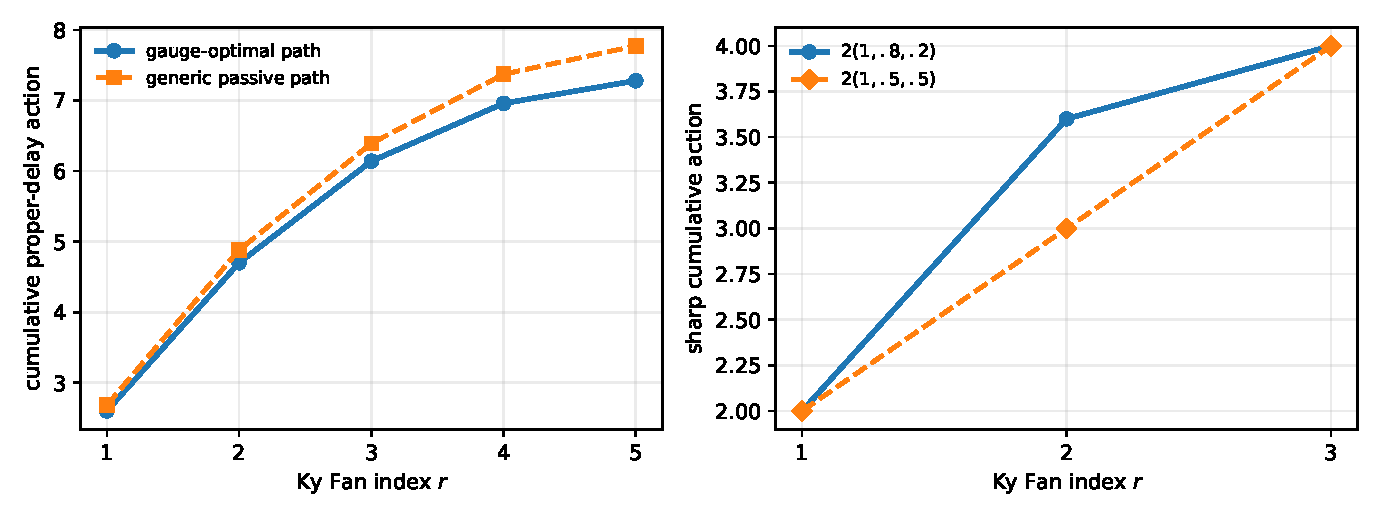
\includegraphics[width=0.78\linewidth]{figures/ky_fan_hierarchy.pdf}
 \caption{The required cumulative action $2\sum_{j\leq r}\beta_j$ is an
 exact lower Lorenz curve.  A coupled-mode family saturates every prefix;
 generic passive motion carries nonnegative surplus resolved by
 \cref{thm:slack}.}
 \label{fig:lorenz}
\end{figure}

\section{Limitations, falsifiers and open directions}

\begin{limitation}[No positivity from unitarity alone]
A general unitary path has Hermitian $Q$ but need not have $Q\succeq0$.
The spectral-spread theorem still holds; the proper-delay and degree
corollaries require positivity.  A measured negative proper delay is a
falsifier for applying those passive-monotone corollaries, not for
\cref{thm:main}.
\end{limitation}

\begin{limitation}[Boundary model]
The theorem constrains a unitary boundary scattering path.  Loss, gain,
unobserved ports and calibration drift must be incorporated through a larger
unitary dilation or an explicit error model.  Treating a visibly contractive
subblock as if it were the full unitary would invalidate the generator
identity.
\end{limitation}

\begin{limitation}[Lower bound, not synthesis classification]
The coupled-mode construction proves all constants optimal but does not
classify every saturating path or solve degree-minimal interpolation for
arbitrary heterogeneous samples.  Equation \eqref{eq:psdslack} provides
necessary near-rigidity conditions, not a complete stability theorem.
\end{limitation}

Promising next questions are: a stability theorem converting small total
slack into distance from the coupled-mode geodesic family; dilation-aware
certificates for measured lossy scattering matrices; and a synthesis theorem
characterizing which proper-delay Lorenz curves above the sharp lower frontier
are realizable by rational inner networks of fixed degree.

\section{Conclusion}

Subspace rotation consumes a spectrum, not a scalar.  The complete law is
$2\beta\prec_w\int\Spr(Q)$: every prefix of canonical-angle motion must be
paid for by the matching prefix of generator spectral spread.  Positive
Wigner--Smith flows turn this into a hierarchy of leading proper-delay
budgets.  The hierarchy is simultaneously sharp, admits an exact three-term
slack decomposition, survives heterogeneous leakage and finite tomography
error, adds over separated switches and closes to an integer McMillan-degree
obstruction for rational passive networks.  It therefore upgrades a trace
memory law into a mode-resolved, experimentally certifiable resource theory.

\section*{Data and code availability}

The manuscript source, frozen JSON certificate, generated figure, independent
verifier, release manifest and continuous-integration workflow are archived at
\href{https://github.com/lluiseriksson/finite-sample-spectral-certificates/releases/tag/v1.4-ky-fan-speed-limits}{the immutable GitHub release}.  The principal claims are proved analytically
in the text; numerical tests are adversarial audits, not substitutes for the
proofs.

\bibliographystyle{plain}
\bibliography{references}

\end{document}
